\chapter{Ciclo de vida}
  Segundo \citeauthor{ihc} (\citeyear{ihc}), Os modelos de ciclo de vida indicam processos que representam conjuntos
  de atividades e suas relações para o projeto de interação, desenvolvimento e distribuição do produto.
  
  As seções seguintes descrevem os modelos de ciclo de vida analisados e apresenta o modelo escolhido para utilização no trabalho.
  \section{Modelo simplificado}
  
  Segundo \citeauthor{ihc} (\citeyear{ihc}), possibilita um número ilimitado de repetição do ciclo, desde que a última 
  atividade sempre seja um teste. É um modelo que foi proposto após observações sobre como a prática do projeto de interação
  acontece na vida real, assim possuindo foco nos usuários e possibilitando que o produto evolua que melhor se adequar a equipe.
  
  Ainda segundo \citeauthor{ihc} (\citeyear{ihc}), o modelo contempla quatro etapas básicas:
  
  \begin{itemize}
  \item Identificar necessidade e estabelecer requisitos;
  \item Construir versões alternativas;
  \item Projeto/re-projeto (protótipos);
  \item Avaliação.
  \end{itemize}  
  
  
  \section{Modelo de engenharia de usabilidade}
  
  Segundo \citeauthor{engusabilidade} (\citeyear{engusabilidade}), visa o desenvolvimento da interação entre o usuário e
  sistema informatizados, tendo por objetivo oferecer algumas técnicas 
  que possam vir a ser utilizadas de modo sistemático para garantir um elevado nível de usabilidade em interfaces. 
  
  %\pagebreak
  
  Esse modelo envolve detalhes rigorosos sobre o desenvolvimento do produto, porém permite que pessoas com pouco 
  conhecimento sobre usabilidade também o utilize \cite{ihc}. 
  Ainda segundo \citeauthor{ihc} (\citeyear{ihc}), o modelo é apoiado na Engenharia de \textit{Software} e se baseia
  em três atividades básicas:
  
  \pagebreak
  
  \begin{itemize}
    \item Análise de Requisitos.

    \item Projeto/teste/desenvolvimento.

    \item Instalação.     
  \end{itemize}  
  
  
  \begin{figure}[!htb]
  \centering
  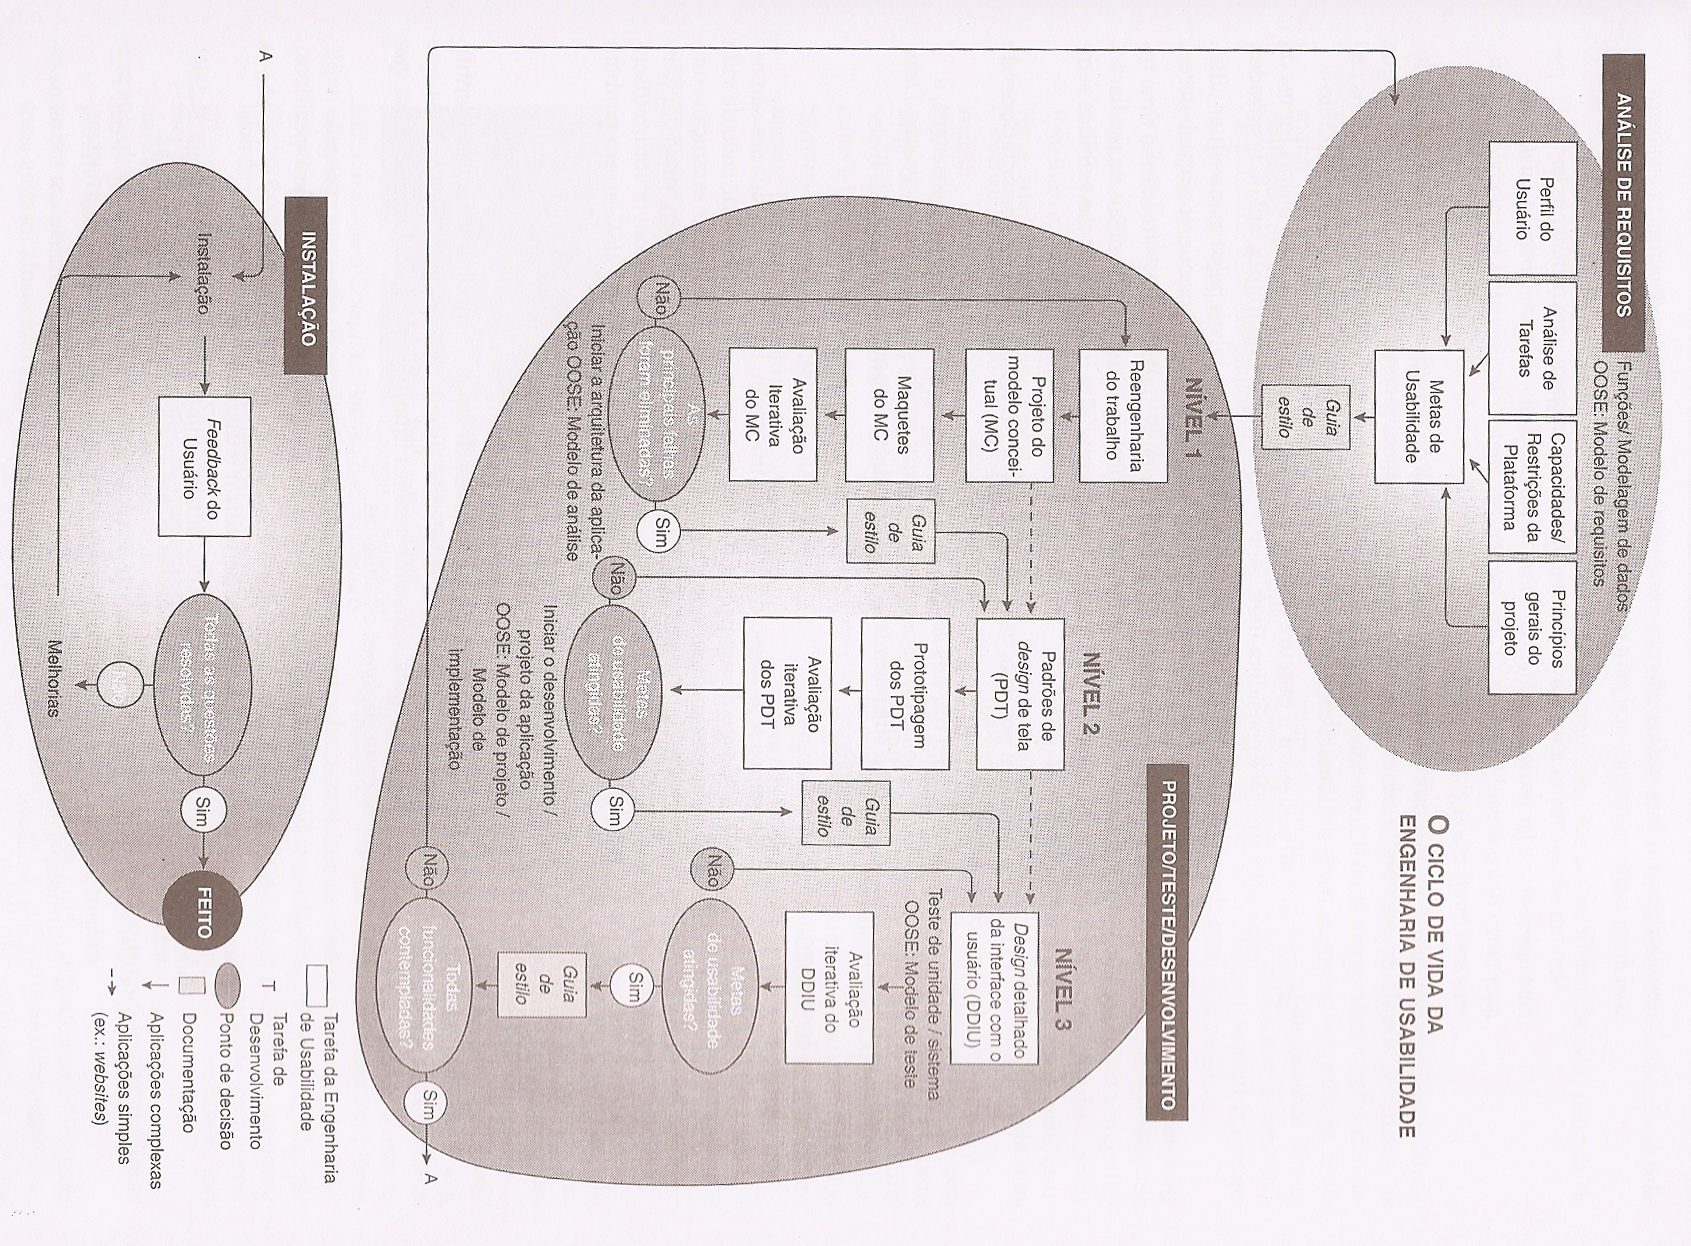
\includegraphics[scale=0.55, angle=90]{figuras/ciclovidaengusabilidade.jpg}
  \caption[Modelo de ciclo de vida da engenharia de usabilidade]{Modelo de ciclo de vida da engenharia de usabilidade \cite{ciclovidaengdeusabilidade}.}
  \end{figure}
%  \vfill
  
  \section{Modelo estrela}
       
       O modelo estrela não deixa especificado um ordenamento das atividades, porém é flexível  de modo que sempre antes de se fazer uma nova atividade 
       seja feita uma avaliação \cite{guiaderef}.
       
       Também segundo \cite{guiaderef}, o modelo apresenta no centro a atividade de avaliação, sendo que esta se interliga a quatro atividades que 
       por sua vez são:
       
       \pagebreak
       
       \begin{itemize}
       \item Implementação.

       \item Análise de tarefas/funcional.

       \item Prototipação.
       
       \item Análise de requisitos/especificação.
       
       \end{itemize}
       
      \begin{figure}[!htb]
      \centering
      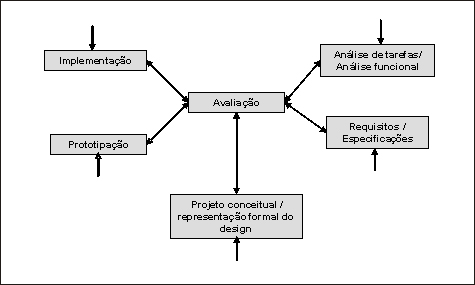
\includegraphics[scale=0.55]{figuras/estrela.jpg}
      \caption[Modelo de ciclo de vida estrela]{Modelo de ciclo de vida estrela \cite{ciclovidaestrela}.}
      \end{figure}
    
    \section{Modelo escolhido}
    
       O modelo escolhido para ser utilizado neste projeto foi o modelo de ciclo de vida estrela.
    
       Mesmo sendo necessário o uso de modelos mais elaborados em projetos maiores, modelos simplificados são os mais práticados na área de Interação 
       Humano Computador \cite{ihc}.
       
       O processo de design seguido foi o modelo Estrela, que envolve as atividades de Implementação, Análise das tarefas, Prototipação, Projeto 
       conceitual e Requisitos, onde é possível começar o desenvolvimento por qualquer uma das atividades e todas as atividades convergem para 
       a avaliação. 
       
       Primeiramente foi feito o projeto conceitual da solução e levantado requisitos iniciais. Logo após, foi iniciada a atividade de prototipação com a 
       confecção do storyboad e o protótipo de papel, onde foram levantados mais requisitos e alguns refinados.
   

  %A Engenharia de Usabilidade (também denominada Design Centrado no Usuário) trata da criação de sistemas melhores através da 
  %compreensão de quem são usuários finais e do envolvimento de usuários nos requisitos, no design de interface do usuário e nos
  %esforços de teste. O modelo que é apoiado na engenharia de software é baseado em três tarefas essenciais: Análise de requisitos
  %e Projeto/teste/desenvolvimento e Instalação.
 % 
  %O ciclo de vida estrela é uma proposta que não especifica um ordenamento das atividades, mas sua flexibilidade exige que uma
  %avaliação sempre seja feita antes de iniciar uma nova atividade. Este modelo inclui a implementação e a análise de tarefas.
  %As  outras atividades vão de encontro com as atividades básicas dos projeto de interação: necessidade e requisitos, versões 
  %alternativas (projeto conceitual) e protótipos e avaliação.
  %
  %O processo de design seguido foi o modelo Estrela, que envolve as atividades de Implementação, Análise das tarefas, Prototipação,
  %Projeto conceitual e Requisitos, onde é possível começar o desenvolvimento por qualquer uma das atividades e todas as atividades
  %convergem para a avaliação.
  %
  %Primeiramente foi feito o projeto conceitual da solução e levantado requisitos iniciais. Logo após, foi iniciada a atividade
  %de prototipação com a confecção do storyboad e o protótipo de papel, onde foram levantados mais requisitos e alguns refinados.